\newpage
\section*{Ignatius Slamet Riyadi: Teladan dari Solo}
\begin{floatingfigure}[r]{2cm}
\begin{center}
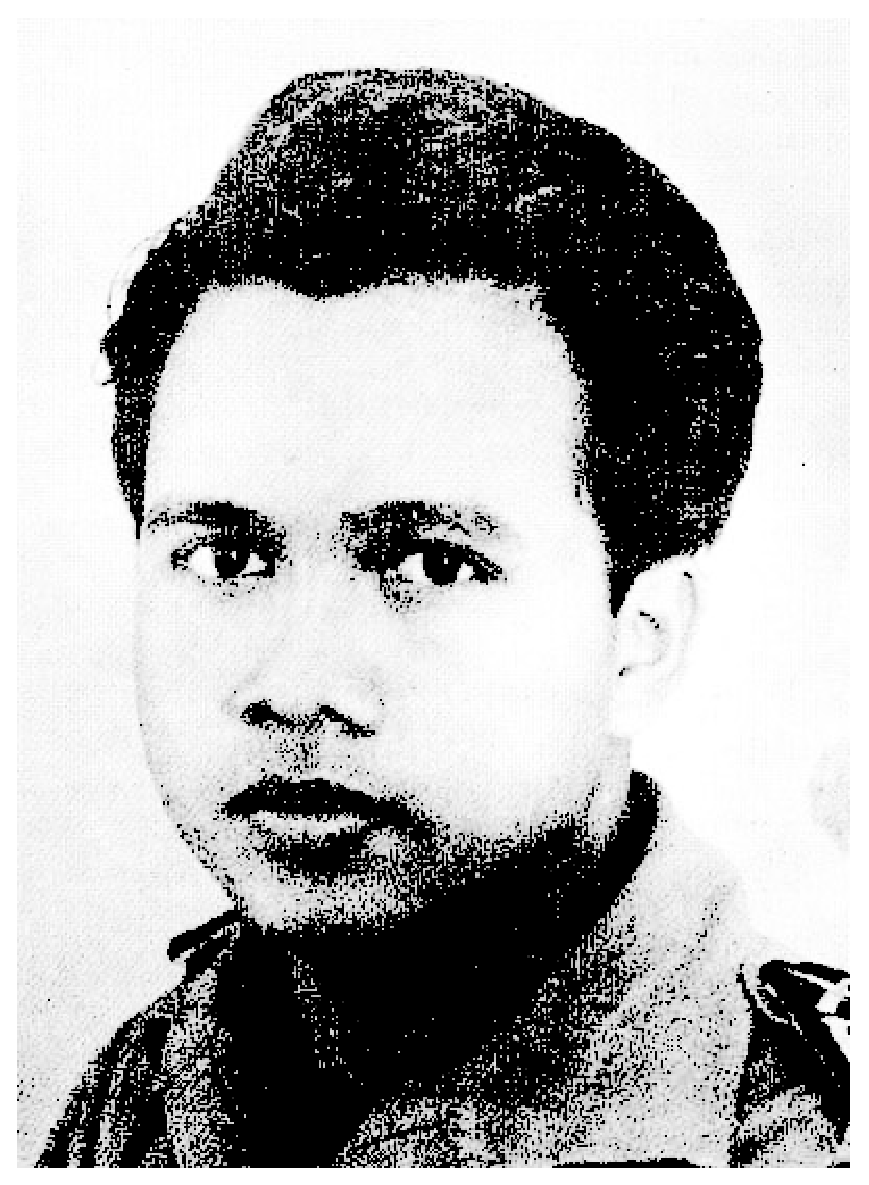
\includegraphics[scale=0.15]{Slamet-riyadi.ps}
\end{center}
\end{floatingfigure}
Salah satu tokoh pahlawan nasional yang berasal dari Solo adalah Ignatius Slamet Riyadi. Sesuai dengan namanya beliau adalah seorang Katolik yang ikut dalam perjuangan kemerdekaan Indonesia. 
Namanya digunakan sebagai nama jalan utama di jantung kota Solo tempat kelahirannya.   
Anak dari Idris Prawiropralebdo, seorang perwira anggota legium Kasunanan Surakarta, yang lahir 26 Juli 1927 ini sangat menonjol kecakapan dan keberaniannya, terutama setelah Jepang bertekuk lutut dan kemerdekaan Indonesia diproklamasikan. 

Ignatius Slamet Rijadi adalah salah seorang di antara ribuan anak muda yang sejak detik pertama Proklamasi Kemerdekaan Indonesia secara sukarela terjun memenuhi panggilan revolusi. Sebagai bekas bintara Kaigun (Angkatan Laut Jepang) yang batal dikirim ke Tokyo karena Perang Pasifik berakhir lebih cepat, Slamet Rijadi kemudian tampil memimpin aksi penyerbuan ke markas Kempeitai (Polisi Rahasia Jepang) di Solo dan menjadi anak zaman. Pertempuran demi pertempuran dilalui Slamet Rijadi, dari mengusir Jepang, melawan Inggris, Belanda, pemberontak Komunis, dan Darul Islam, hingga menumpas Republik Maluku Selatan. Dia gugur pada usia 23 tahun dengan pangkat Letnan Kolonel sebagai Komandan Operasi Maluku Selatan akibat tembakan seorang sniper di depan Fort Victoria, Ambon, Maluku. Sebutan Pahlawan Nasional sekaligus anugerah Bintang Mahaputera Adipradana kepada Brigadir Jenderal (Anumerta) Ign. Slamet Rijadi disampaikan oleh Presiden Susilo Bambang Yudhoyono awal November 2007 \textit{"untuk tindak kepahlawanan dalam perjuangan merebut, membela dan mempertahankan negara dan bangsa, sehingga bisa jadi teladan bagi seluruh masyarakat Indonesia."}

\subsection*{Kepahlawanan}

Pada suatu peristiwa saat akan diadakannya peralihan kekuasaan di Solo oleh Jepang yang dipimpin oleh Tyokan Watanabe yang merencanakan untuk mengembalikan kekuasaan sipil kepada kedua kerajaan yang berkedudukan di Surakarta, yaitu Kasunanan dan Praja Mangkunagaran, akan tetapi rakyat tidak puas. Para pemuda telah bertekad untuk mengadakan perebutan senjata dari tangan Jepang, maka rakyat mengutus Muljadi Djojomartono dan dikawal oleh pemuda Suadi untuk melakukan perundingan di markas Ken Pei Tai (polisi militer Jepang) yang dijaga ketat. Tetapi sebelum utusan tersebut tiba di markas, seorang pemuda sudah berhasil menerobos kedalam markas dengan meloncati tembok dan membongkar atap markas Ken Pei Tai, tercenganglah pihak Jepang, pemuda itu bernama Slamet Riyadi.


\subsection*{Karir militer}

Pada tahun 1940, ia menyelesaikan pendidikan di HIS, ke Mulo Afd. B dan kemudian dilanjutkan ke Pendidikan Sekolah Pelayaran Tinggi, dan memperoleh ijasah navigasi laut dengan peringkat pertama dan mengikuti kursus tambahan dengan menjadi navigator pada kapal kayu yang berlayar antar pulau Nusantara. Setelah pasukan Jepang, mendarat di Indonesia melalui Merak, Indramayu dan dekat Rembang pada tanggal 1 Maret 1942 dengan kekuatan 100.000 orang, dan walaupun memperoleh perlawanan dari Hindia Belanda,  tetapi dalam waktu singkat yaitu pada tanggal 5 dan 7 Maret 1942,  Kota Solo dan Yogyakarta jatuh ketangan Jepang.

Slamet Riyadi merasa terpanggil membela ibu pertiwi, dan menjelang proklamasi 1945,  ia mengobarkan pemberontakan dan melarikan sebuah kapal kayu milik Jepang, usaha Ken Pei Tai untuk menangkapnya tidak pernah berhasil,  bahkan setelah Jepang bertekuk lutut. Slamet Rijadi berhasil menggalang para pemuda, menghimpun kekuatan pejuang dari pemuda-pemuda terlatih eks Peta/Heiho/Kaigun dan merekrutnya dalam kekuatan setingkat Batalyon,  yang dipersiapkan untuk mempelopori perebutan kekuasaan politik dan militer di kota Solo dari tangan Jepang ( Slamet Riyadi diangkat sebagai Komandan Batalyon Resimen I Divisi X ).

Dalam perkembangannya terjadi pergantian pimpinan militer,  Divisi X dirubah menjadi Divisi IV, dengan Panglimanya Mayor Jenderal Soetarto dan divisi ini dikenal dengan nama Divisi Penembahan Senopati, yang membawahi 5 Brigade tempur . Diantaranya Brigade V dibawah pimpinan Suadi dan mempunyai Batalyon XIV dibawah komando Mayor Slamet Rijadi,  yang merupakan kesatuan militer yang dibanggakan. Pasukannya terkenal dengan sebutan anak buah "Pak Met" . Selama agresi Belanda II,  pasukannya sangat aktif melakukan serangan gerilya terhadap kedudukan militer Belanda, pertempuran demi pertempuran membuat sulit pasukan Belanda dalam menghadapi taktik gerilya yang dijalankan Slamet Riyadi. 

Namanya mulai disebut-sebut karena hampir di-setiap peristiwa perlawanan di kota Solo selalu berada dalam komandonya.

Sewaktu pecah pemberontakan PKI-Madiun, batalyon Slamet Rijadi sedang berada diluar kota Solo, yang kemudian diperintahkan secara langsung oleh Gubernur Militer II - Kolonel Gatot Subroto untuk melakukan penumpasan ke arah Utara, berdampingan dengan pasukan lainnya, operasi ini berjalan dengan gemilang.

Dalam palagan perang kemerdekaan II, Slamet Rijadi dinaikkan pangkatnya menjadi Letnan Kolonel, dengan jabatan baru Komandan "Wehrkreise I" ( Penembahan Senopati )yang meliputi daerah gerilya Karesidenan Surakarta, dan dibawah komando Gubernur Militer II pada Divisi II,  Kolonel Gatot Subroto. Dalam perang kemerdekaan II inilah Let.Kol. Slamet Rijadi, membuktikan kecakapannya sebagai prajurit yang tangguh dan sanggup mengimbangi kepiawaian komandan Belanda lulusan Sekolah Tinggi Militer di Breda Nederland. Siang dan malam anak buah Overste (setingkat Letnan Kolonel ). Van Ohl digempur habis-habisan, dengan penghadangan, penyergapan malam, sabotase . Puncaknya ketika Let.Kol Slamet Riyadi mengambil prakarsa mengadakan "Serangan Umum Kota Solo" yang dimulai tanggal 7 Agustus 1949, selama empat hari empat malam. Serangan itu membuktikan kepada Belanda, bahwa gerilya bukan saja mampu melakukan penyergapan atau sabotase, tetapi juga mampu melakukan serangan secara frontal ketengah kota Solo yang dipertahankan dengan pasukan kavelerie, persenjataan berat-artileri, pasukan infantri dan komando yang tangguh. Dalam pertempuran selama empat hari tersebut, 109 rumah penduduk porak poranda, 205 penduduk meninggal karena aksi teror Belanda,  7 serdadu Belanda tertembak dan 3 orang tertawan sedangkan dipihak TNI 6 orang gugur.

Setelah terjadi gencatan senjata,  dan pada waktu penyerahan kota Solo kepangkuan Republik Indonesia,  dari pihak Belanda diwakili oleh "Overste Van Ohl" sedangkan dari pihak R.I oleh Let.Kol. Slamet Riyadi. Ov.Van Ohl demikian terharu, bahwa Let. Kol. Slamet Riyadi yang selama ini dicari-carinya ternyata masih sangat muda . " Oooh ...Overste tidak patut menjadi musuh-ku.....", Overste pantas menjadi anakku, tetapi kepandaiannya seperti ayahku.

Pada akhir tahun 1949, sebagai penganut agama Katolik, Slamet Riyadi di baptis dengan nama Ignatius di Gereja Santo Antonius Purbayan Solo. Pada tanggal 10 Juli 1950, Letnan Kolonel Ignatius Slamet Rijadi, berangkat dengan kapal Waikalo dan memimpin batalyon 352 untuk bergabung dengan pimpinan umum operasi - Panglima TT VII - Kolonel Kawilarang, dalam penugasan menumpas pemberontakan Kapten Andi Aziz di Makasar dan pemberontakan Republik Maluku Selatan (RMS) yang dipelopori oleh Dr. Soumokil dan kawan-kawan.

\subsection*{Riwayat Perjuangan}

\begin{tabular}{cp{9cm}}
1940&Sekolah Tinggi Pelayaran Rekrutmen Pemuda oleh tentara Jepang\\ 
1943&Navigator kapal kayu Pemberontakan kapal,milik Jepang \\
1945&Dan.Yon.Res.I, Divisi I Perang di Krsd. Solo melawan Jepang \& Belanda\\ 
1945&Dan.Yon.Res.I, Divisi I Penumpasan pemberontakan PKI Madiun \\
1948&Dan.Wehrkreise I Perang Kemerdekaan II, Serangan Umum Solo \\
1949&Wakil Pemerintah RI Penyerahan Kota Solo \\
1949&Komando Yon.352 Mendukung Div.Siliwangi menumpas APRA di Jabar.\\ 
1949&Wakil.Panglima TT VII. Penumpasan Pemberontakan di Makasar, RMS Ambon \\
1950&Wakil.Panglima TT VII. \\
1950&Gugur di gerbang benteng Victoria, Ambon 4-11-1950 \\

1950&Brigadir Jendral Anumerta Kenaikan pangkat atas jasa almarhum\\ 
2007&mendapat penghormatan sebagai Pahlawan Nasional. \\
2007&dibangun Patung Ignatius Slamet Riyadi di bundaran Gladak, Solo.\\
\end{tabular}